%!TEX TS-program = xelatex
%!TEX encoding = UTF-8 Unicode

%! xelatex thesis.tex
%! makeindex thesis.nlo -s nomencl.ist -o thesis.nls

\documentclass{hi-thesis} 
\usepackage{ifthen}
\usepackage{float}
\usepackage{morefloats}

\usepackage{footnote}
\usepackage[bottom,perpage,symbol*]{footmisc}

\newcommand{\tcr}[1]{{\color{red} #1}}
\newcommand{\tcb}[1]{{\color{blue} #1}}
\newcommand{\tcg}[1]{{\color{green} #1}}
\newcommand{\Alice}{Alice}
\newcommand{\fullnameAlice}{Adaptive Learning Intelligent Composite rulEs}

\newcommand*\blankpage{%
	\newpage	
	\topskip0pt
	\vspace*{\fill}
	\centering This page is intentionally left blank.
	\vspace{\fill}			
}

 % put your own shorthand declarations in this document
\bibinput{papers/papers} % put only *your* publications here
\begin{document}
\printmode{final} % draft or final - case sensitive

% Front matter and dependencies defined
\printFrontMatter{This is not for you} % insert your dedication here

% Main matter, include each chapter...
\prologue
\HeaderQuote{What is the use of a book, without pictures or conversations?}{Alice} 

\chapter{Something different }

\newthought{There's something to be said} for having a good opening line. Morbi commodo, ipsum sed pharetra gravida, orci  $x = 1/\alpha$ magna rhoncus neque, id pulvinar odio lorem non turpis. Nullam sit amet enim. Suspendisse id velit vitae ligula volutpat condimentum. Aliquam erat volutpat. Sed quis velit. Nulla facilisi. Nulla libero. Vivamus pharetra posuere sapien. Nam consectetuer. Sed aliquam, nunc eget euismod ullamcorper, lectus nunc ullamcorper orci, fermentum bibendum enim nibh eget ipsum. Donec porttitor ligula eu dolor. Maecenas vitae nulla consequat libero cursus venenatis. Nam magna enim, accumsan eu, blandit sed, blandit a, eros.
$$\zeta = \frac{1039}{\pi}$$
For an example of a full page figure, see Fig.~\ref{fig:myFullPageFigure}.

Lorem ipsum dolor sit amet, consectetuer adipiscing elit. Morbi commodo, ipsum sed pharetra gravida, orci magna rhoncus neque, id pulvinar odio lorem non turpis. Nullam sit amet enim. Suspendisse id velit vitae ligula volutpat condimentum. Aliquam erat volutpat. Sed quis velit. Nulla facilisi. Nulla libero. Vivamus pharetra posuere sapien. Nam consectetuer. Sed aliquam, nunc eget euismod ullamcorper, lectus nunc ullamcorper orci, fermentum bibendum enim nibh eget ipsum. Donec porttitor ligula eu dolor. Maecenas vitae nulla consequat libero cursus venenatis. Nam magna enim, accumsan eu, blandit sed, blandit a, eros.

\begin{table}
\[\begin{array}{cc} 1 & 3 \\ 2 & 4 \end{array}\]
\caption{bla}
\end{table}

Quisque facilisis erat a dui. Nam malesuada ornare dolor. Cras gravida, diam sit amet rhoncus ornare, erat elit consectetuer erat, id egestas pede nibh eget odio. Proin tincidunt, velit vel porta elementum, magna diam molestie sapien, non aliquet massa pede eu diam. Aliquam iaculis. Fusce et ipsum et nulla tristique facilisis. Donec eget sem sit amet ligula viverra gravida. Etiam vehicula urna vel turpis. Suspendisse sagittis ante a urna. Morbi a est quis orci consequat rutrum. Nullam egestas feugiat felis. Integer adipiscing semper ligula. Nunc molestie, nisl sit amet cursus convallis, sapien lectus pretium metus, vitae pretium enim wisi id lectus. Donec vestibulum. Etiam vel nibh. Nulla facilisi. Mauris pharetra. Donec augue. Fusce ultrices, neque id dignissim ultrices, tellus mauris dictum elit, vel lacinia enim metus eu nunc.

\section{First Paragraph}
And now I begin my first chapter here ...

Here is an equation\footnote{the notation is explained in the nomenclature section :-)}:
\begin{eqnarray}
CIF: \hspace*{5mm}F_0^j(a) &=& \frac{1}{2\pi \iota} \oint_{\gamma} \frac{F_0^j(z)}{z - a} dz
\end{eqnarray}
\nomenclature[zcif]{$CIF$}{Cauchy's Integral Formula}                  % first letter Z is for Acronyms 
\nomenclature[aF]{$F$}{complex function}                               % first letter A is for Roman symbols
\nomenclature[gp]{$\pi$}{ $\simeq 3.14\ldots$}                         % first letter G is for Greek Symbols
\nomenclature[gi]{$\iota$}{unit imaginary number $\sqrt{-1}$}          % first letter G is for Greek Symbols
\nomenclature[gg]{$\gamma$}{a simply closed curve on a complex plane}  % first letter G is for Greek Symbols
\nomenclature[xi]{$\oint_\gamma$}{integration around a curve $\gamma$} % first letter X is for Other Symbols
\nomenclature[rj]{$j$}{superscript index}                              % first letter R is for superscripts
\nomenclature[s0]{$0$}{subscript index}                                % first letter S is for subscripts

Pellentesque habitant morbi tristique senectus et netus et malesuada fames ac turpis egestas. Vestibulum tortor quam, feugiat vitae, ultricies eget, tempor sit amet, ante. Donec eu libero sit amet quam egestas semper. Aenean ultricies mi vitae est. Mauris placerat eleifend leo. Quisque sit amet est et sapien ullamcorper pharetra. Vestibulum erat wisi, condimentum sed, commodo vitae, ornare sit amet, wisi. Aenean fermentum, elit eget tincidunt condimentum, eros ipsum rutrum orci, sagittis tempus lacus enim ac dui. Donec non enim in turpis pulvinar facilisis. Ut felis.

\begin{figure}  
\includegraphics[width=\textwidth]{figures/fig1}
\caption[Short figure name.]{This is a figure that floats inline and here is its caption.
\label{fig:myInlineFigure}}
\end{figure}



\begin{FPfigure}  
\includegraphics[width=\textwidth]{figures/fullpage}
\caption[Short figure name.]{This is a full page figure using the FPfigure command. It takes up the whole page and the caption appears on the preceding page. Its useful for large figures. Harvard's rules about full page figures are tricky, but you don't have to worry about it because we took care of it for you. For example, the full figure is supposed to have a title in the same style as the caption but without the actual caption. The caption is supposed to appear alone on the preceding page with no other text. You do't have to worry about any of that. We have modified the fltpage package to make it work. This is a lengthy caption and it clearly would not fit on the same page as the figure. Note that you should only use the FPfigure command in instances where the figure really is too large. If the figure is small enough to fit by the caption than it does not produce the desired effect. Good luck with your thesis. I have to keep writing this to make the caption really long. LaTex is a lot of fun. You will enjoy working with it. Good luck on your post doctoral life! I am looking forward to mine. \label{fig:myFullPageFigure}}
\end{FPfigure}


Nulla facilisi. In vel sem. Morbi id urna in diam dignissim feugiat. Proin molestie tortor eu velit. Aliquam erat volutpat. Nullam ultrices, diam tempus vulputate egestas, eros pede varius leo, sed imperdiet lectus est ornare odio. Lorem ipsum dolor sit amet, consectetuer adipiscing elit. Proin consectetuer velit in dui. Phasellus wisi purus, interdum vitae, rutrum accumsan, viverra in, velit. Sed enim risus, congue non, tristique in, commodo eu, metus. Aenean tortor mi, imperdiet id, gravida eu, posuere eu, felis. Mauris sollicitudin, turpis in hendrerit sodales, lectus ipsum pellentesque ligula, sit amet scelerisque urna nibh ut arcu. Aliquam in lacus. Vestibulum ante ipsum primis in faucibus orci luctus et ultrices posuere cubilia Curae; Nulla placerat aliquam wisi. Mauris viverra odio. Quisque fermentum pulvinar odio. Proin posuere est vitae ligula. Etiam euismod. Cras a eros.


% Back matter
\HeaderQuote{A cat may look at a king. I've read that in some book, but I don't 
remember where.}{Alice}

\bibliographystyle{abbrvnat} 
\bibliography{papers/references}
\addcontentsline{toc}{chapter}{\bibname}

\appendix
\HeaderQuote{What is the use of a book, without pictures or conversations?}{Alice}

\chapter{Test function suite}\label{app:fun} \todo[color=green!40]{\cref{app:fun} Unfinished}
\FirstSentence{T}{est functions $f$ used} in~\cref{ch:surrogates} are defined $f:\mathbb{R}^d\mapsto\mathbb{R}$.

\todo[inline]{All benchmark functions with the exception of ?? are described in [?]. They are summarized here for completeness. The original sources of the functions are also cited.
	\url{https://notendur.hi.is/tpr/software/sres/testfcn.pdf}
}

\section{Sphere }\label{app:fun:sphere}
Sphere function is a convex and unimodal function (cf.~\cref{fig:fun:sphere}). Sphere function is defined as follows,
\begin{eqnarray}
	f_{\textrm{Sphere}}(\vec{x})&=&\sum_{i=1}^d x_i^2
\end{eqnarray} where $\vec{x}\in[-3,7]^d$.
It has a global minimum at $\vec{x}=\textbf{0}$ where $f_{\textrm{Sphere}}(\textbf{0})=0$. 

\section{Noisy sphere}\label{app:fun:nsphere}
Noisy sphere function is the sphere function from~\cref{app:fun:sphere} where a Gaussian noise has added to perturb the sphere (cf.~\cref{fig:fun:nsphere} where $\epsilon=0.1$). Noisy sphere function is defined as follows,
\begin{eqnarray}
	f_{\textrm{NoisySphere}}(\vec{x})&=&f_{\textrm{Sphere}}(\vec{x})\left(1+\epsilon\mathcal{N}(0,1)\right)
\end{eqnarray} where $\vec{x}\in[-3,7]^d$.
It has a global minimum at $\vec{x}=\textbf{0}$ where $f_{\textrm{NoisySphere}}(\textbf{0})=0$.

\section{Schwefel}\label{app:fun:schwefel}
Schwefel is ... (cf.~\cref{fig:fun:schwefel}). Schwefel function is defined as follows,
\begin{eqnarray}
	f_{\textrm{Schwefel}}(\vec{x})&=&\sum_{i=1}^d\left(\sum_{j=1}^i x_j\right)^2
\end{eqnarray} where $\vec{x}\in[-10,10]^d$.
It has a global minimum at $\vec{x}=\textbf{0}$ where $f_{\textrm{Schwefel}}(\textbf{0})=0$.

\section{Ellipsoid}\label{app:fun:ellipsoid}
Ellipsoid is ... (cf.~\cref{fig:fun:ellipsoid}). Ellipsoid function is defined as follows,
\begin{eqnarray}f_{\textrm{Ellipsoid}}(\vec{x})=\sum_{i=1}^d \left(100^{\frac{i-1}{d-1}}x_i\right)^2
\end{eqnarray} where $\vec{x}\in[-3,7]^d$.
It has a global minimum at $\vec{x}=\textbf{0}$ where $f_{\textrm{Ellipsoid}}(\textbf{0})=0$.

\section{Rosenbrock}\label{app:fun:rosen}
Rosenbrock function is a non-convex function, where the global minimum is inside a long, narrow, parabolic shaped flat valley (cf.~\cref{fig:fun:rosen}). To find the valley is trivial. To converge to the global minimum, however, is difficult. Rosenbrock function is defined as follows,
\begin{eqnarray}
	f_{\textrm{Rosenbrock}}(\vec{x})&=&\sum_{i=1}^{d-1} \left(100\cdot(x_i^2-x_{i+1})^2+(x_i-1)^2\right)
\end{eqnarray} where $\vec{x}\in[-5,5]^d$. 
It has a global minimum at $\vec{x}=\textbf{1}$ where $f_{\textrm{Rosenbrock}}(\textbf{1})=0$.

\section{Ackley}\label{app:fun:ackley}
Ackley function is a non-convex function, where the function is a fairly difficult problem due to its large search space and its large number of local minima (cf.~\cref{fig:fun:ackley}). Ackley function is defined as follows,
\begin{eqnarray}
	f_{\textrm{Ackley}}(\vec{x})&=&20-20\cdot\exp\left(-0.2\sqrt{\frac{1}{n}\sum_{i=1}^d x_i^2}\right)
	\\&&+e-\exp\left(\frac{1}{2}\sum_{i=1}^d \cos(2\pi x_i)\right) \nonumber
\end{eqnarray} where $\vec{x}\in[1,30]^d$.
It has a global minimum at $\vec{x}=\textbf{0}$ where $f_{\textrm{Ackley}}(\textbf{0})=0$.

\section{Rastrigin}\label{app:fun:rastrigin}
Rastrigin function is based on the sphere function from~\cref{app:fun:sphere} with the addition of cosine modulation in order to produce frequent local minima (cf.~\cref{fig:fun:rastrigin}). Thus, the test function is highly multimodal. However, the location of the minima are regularly distributed. Rastrigin function is defined as follows,
\begin{eqnarray}
	f_{\textrm{Rastrigin}}(\vec{x})&=&10n+\sum_{i=1}^d \left(x_i^2-10\cos(2\pi x_i)\right)
\end{eqnarray} where $\vec{x}\in[1,5]^d$. 
It has a global minimum at $\vec{x}=\textbf{0}$ where $f_{\textrm{Rastrigin}}(\textbf{0})=0$.

\begin{figure}\centering
	\begin{subfigure}{0.37\textwidth}
		\centering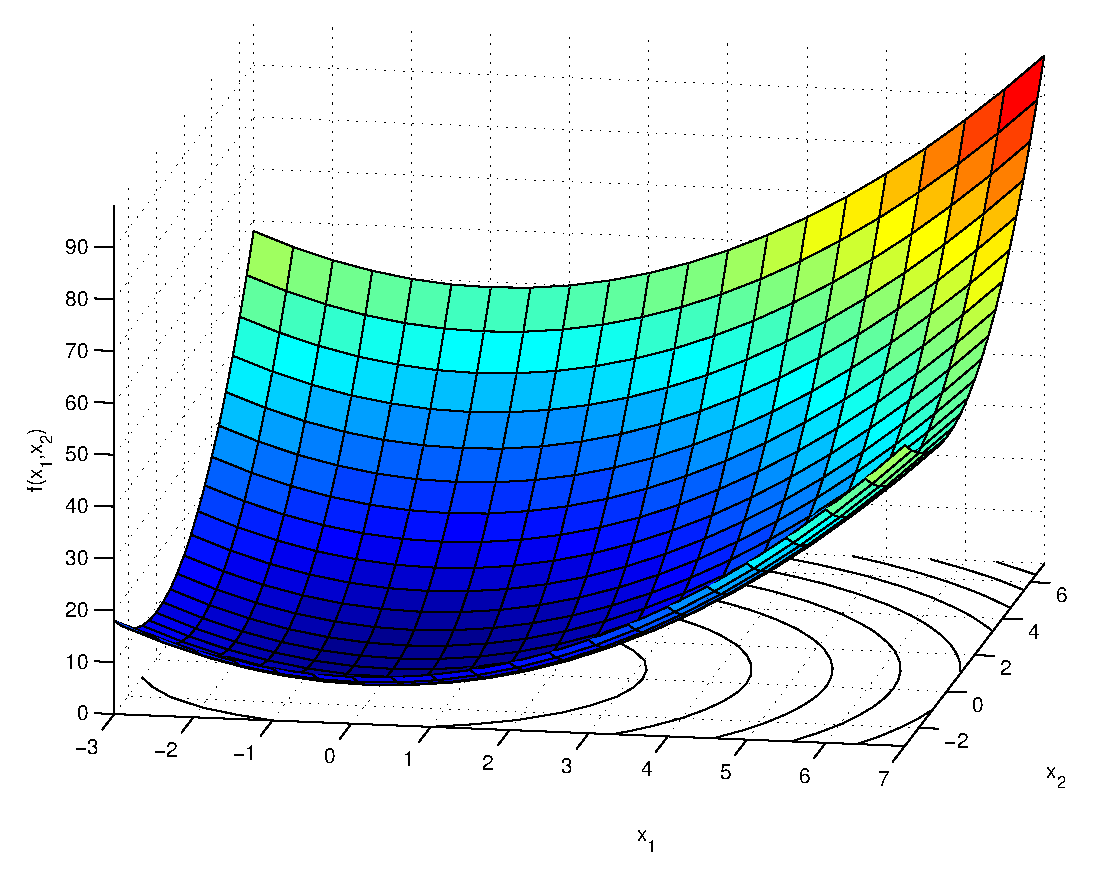
\includegraphics{fun/sphere}
		\caption{Sphere function}\label{fig:fun:sphere}
	\end{subfigure}
	\quad
	\begin{subfigure}{0.37\textwidth}
		\centering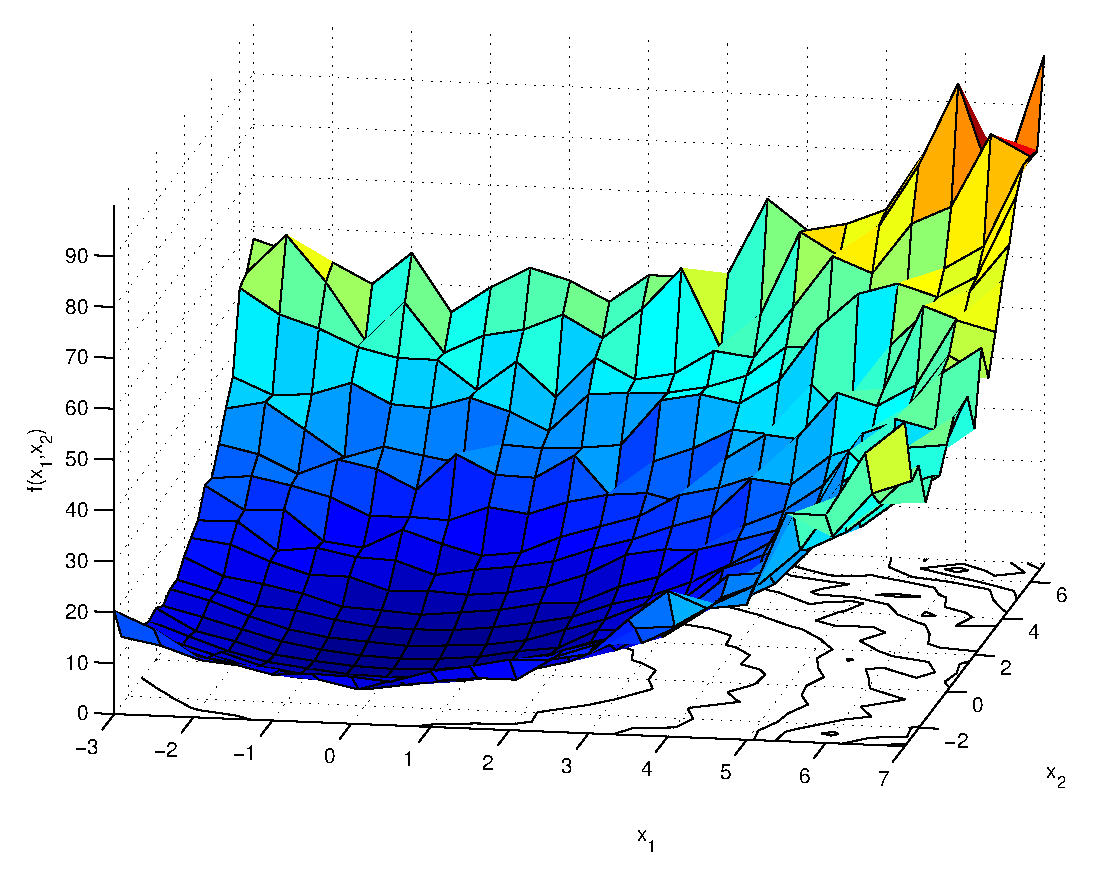
\includegraphics{fun/nsphere}
		\caption{Noisy sphere (with $\epsilon=0.1$)}\label{fig:fun:nsphere}
	\end{subfigure}
	\\
	\begin{subfigure}{0.37\textwidth}
		\centering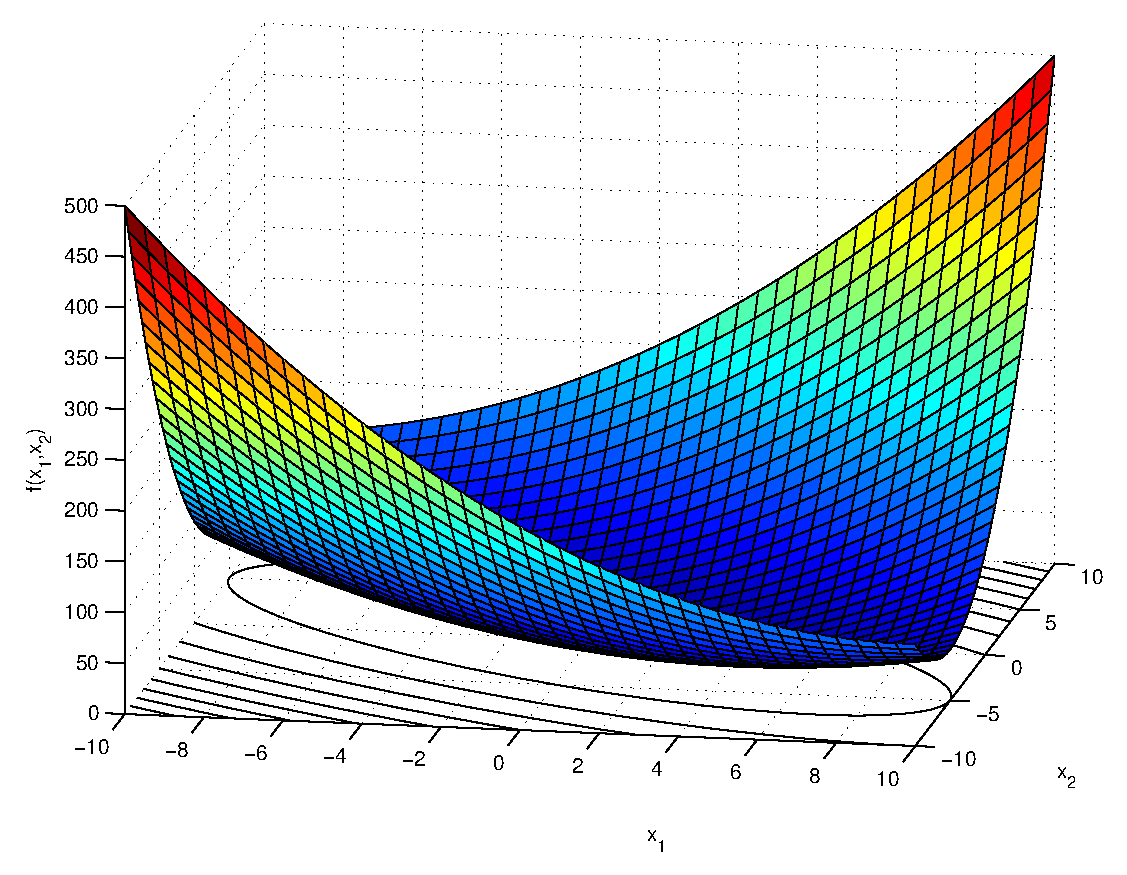
\includegraphics{fun/schwefel}
		\caption{Schwefel}\label{fig:fun:schwefel}
	\end{subfigure}
	\quad
	\begin{subfigure}{0.37\textwidth}
		\centering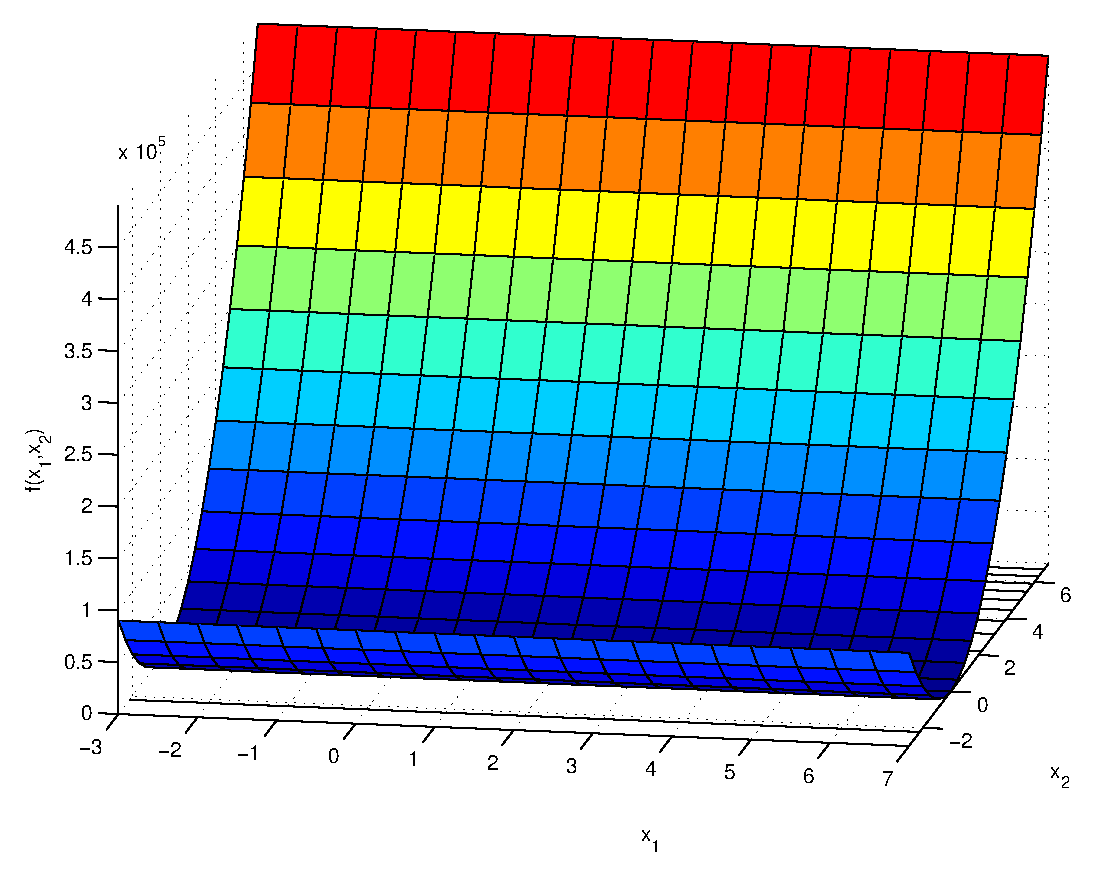
\includegraphics{fun/ellipsoid}
		\caption{Ellipsoid}\label{fig:fun:ellipsoid}
	\end{subfigure}
	\\
	\begin{subfigure}{0.37\textwidth}
		\centering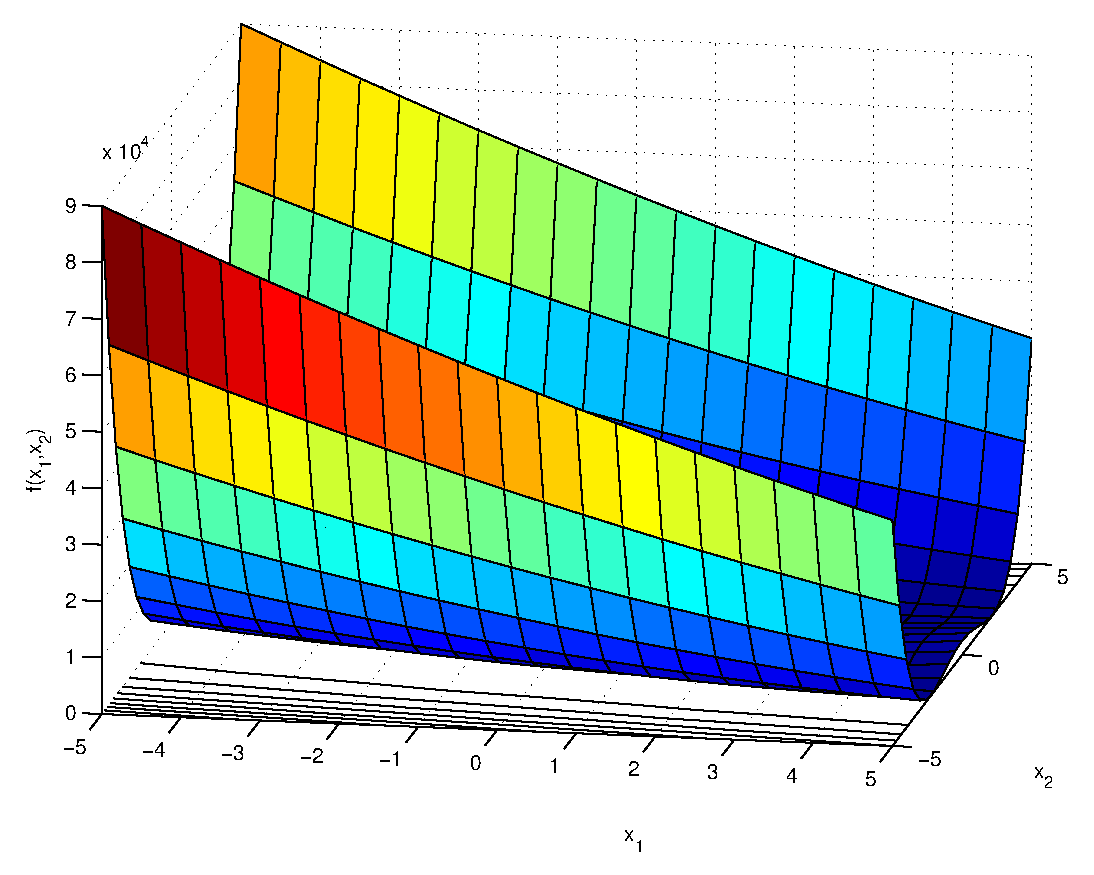
\includegraphics{fun/rosen}
		\caption{Rosenbrock}\label{fig:fun:rosen}
	\end{subfigure}
	\quad
	\begin{subfigure}{0.37\textwidth}
		\centering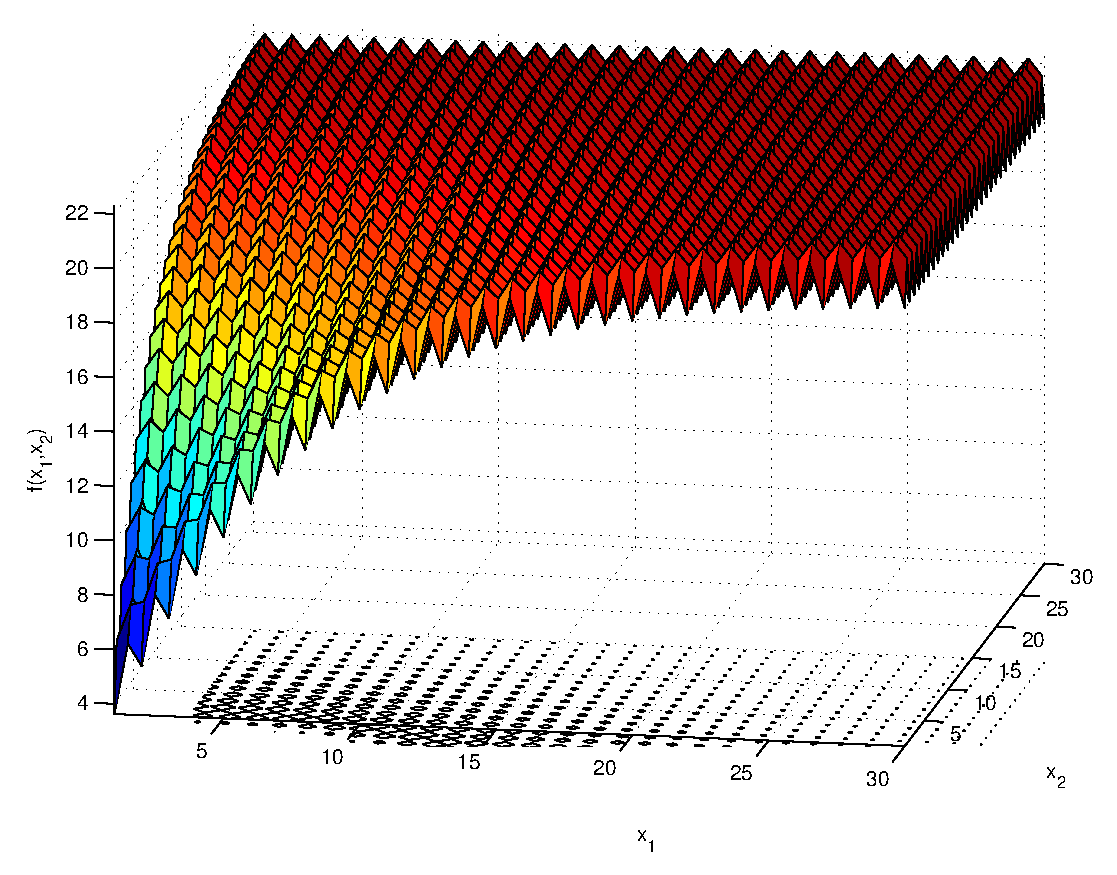
\includegraphics{fun/ackley}
		\caption{Ackley}\label{fig:fun:ackley}
	\end{subfigure}
	\\
	\begin{subfigure}{0.37\textwidth}
		\centering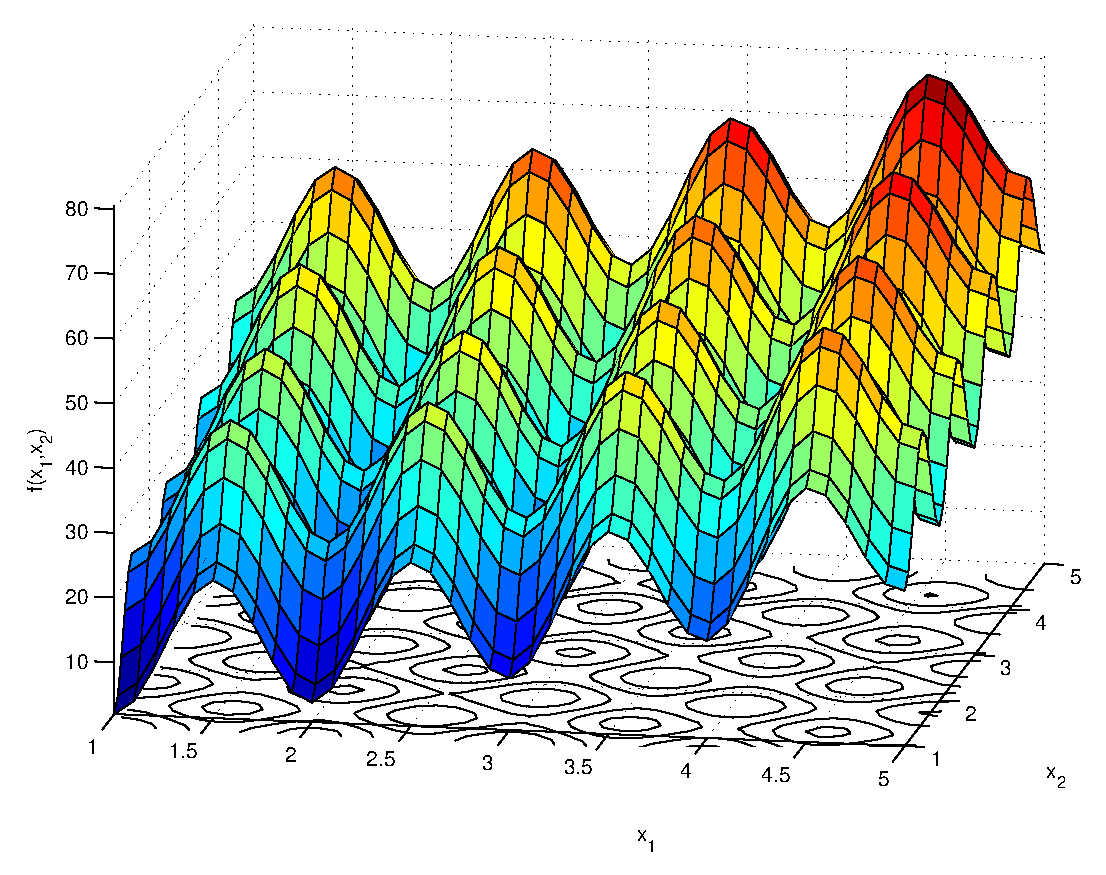
\includegraphics{fun/rastrigin}
		\caption{Rastrigin}\label{fig:fun:rastrigin}
	\end{subfigure}
	\caption{Test function suite of two variables in 3D.}
\end{figure}





 % test function suite

\papers % this includes all our published papers from endmatter/papers

\colophon
\end{document}
